%% ============================================================

\clearpage
From this point on is old stuff
\section{FRAMEWORK}\label{s:framework}

%% ============================================================

\subsection{\chronomod{Sensor}}\label{s:ChSensor}

\chrono{} and \synchrono{} and \chronomod{Vehicle} \chronomod{Sensor} is a Project \chrono{} submodule for sensing simulation. Supported sensors include camera, lidar, \gps{}, and \imu{}. Exteroceptive sensing (camera, \lidar{}) leverages headless, off-screen ray-tracing support via \optix{}. \chronomod{Sensor} seeks to generate realistic data that is equivalent to data from its physical counterpart. To this end, \chronomod{Sensor} supports modeling and simulation of the noise and distortion observed on the data streams of physical sensors. Examples of \chronomod{Sensor} used to simulate a scaled autonomous vehicle navigating a closed course are shown below.

\begin{figure}
	\centering
	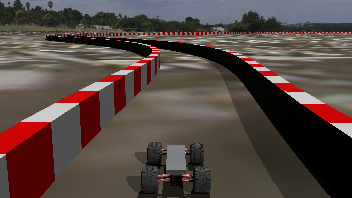
\includegraphics[width=0.8\columnwidth]{Figs/AV-third-person.png}
	\caption{{\small Third person perspective of scaled autonomous vehicle navigating a course using a simulated camera and \lidar{}.}}   
	\label{fig:avthirdperson}
\end{figure}

\begin{figure}
	\centering
	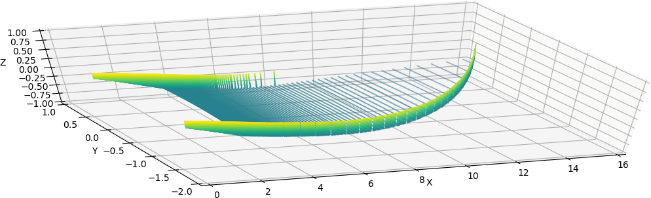
\includegraphics[width=0.8\columnwidth]{Figs/AV-lidar.png}
	\caption{{\small Lidar data showing the course from the perspective of the virtual vehicle. The data is used in the control stack to detect the barriers and determine the desired path.}}   
	\label{fig:avlidar}
\end{figure}

\begin{figure}
	\centering
	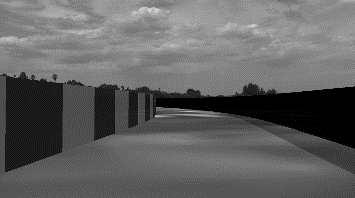
\includegraphics[width=0.8\columnwidth]{Figs/AV-greyscale.png}
	\caption{{\small Image from a simulated grayscale camera mounted to the front of the scaled autonomous vehicle.}}   
	\label{fig:avgreyscale}
\end{figure}

%%============================================================

\subsection{\pychrono{} and \gymchrono{}}\label{s:pyandgym}

\pychrono{} is a package that provides Python bindings for the \chrono{} \api{}. Using an interface compiler (SWIG), the vast majority of the \chrono{} \api{} (multibody dynamics, Vehicle, Sensor, \fea{}, etc.) can be directly accessed from Python. Beyond ease of use, the Python wrapping allows interfacing \chrono{} and ML frameworks for training neural networks. \gymchrono{} provides a set of Robotics and Autonomous Driving environments leveraging \chrono{} for physics simulation and OpenAI gym support for Reinforcement Learning baselines and tools for scalable training.

%%============================================================

\subsection{\synchrono{}}\label{s:synchrono}

\synchrono{} is a software component built on top of \chrono{} that allows for a distributed-memory execution of simulation scenarios that include tens of agents. It builds off the Message Passing Interface (\mpi{}), which allows the toolset to have multiple instances of \chrono{} run simultaneously on a supercomputer/cluster/multi-core setup to allow for the distributed simulation of multiple agents (robots, tracked vehicles, wheeled vehicles, etc.) The paradigm embraced is that of running one \chrono{} agent simulation as one \mpi{} rank, with multiple ranks, say N, communicating through messages to maintain a space and time coherent solution for the N agents participating in the study. This multi-agent form of simulation distribution is possible because of the largely decoupled nature of mobility scenarios. Each agent runs in its own rank and interfaces with its dedicated control stack for software-in-the-loop control. The control stack is fed synthetic data generated by \chronomod{Sensor} and acts upon the environment through \chronomod{Vehicle} control input (throttle, steering, braking, etc.) This “one agent-to-one \chrono{} system” mapping ensures scalability over a monolithic \chrono{} system as shown in the center picture below. The control algorithm or “brain” for each agent is also configurable and can vary from complex algorithms that collect a variety of sensor data, to controls based on empirical models, to human-driven control in scenarios that are simple enough to allow real-time simulation.

\begin{figure}
	\centering
	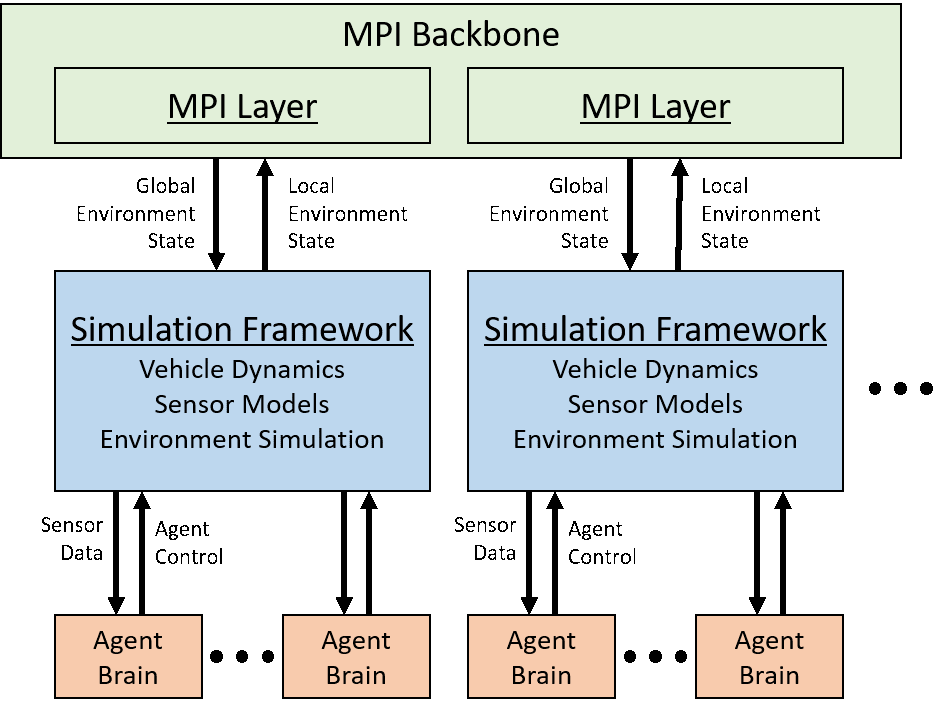
\includegraphics[width=0.8\columnwidth]{Figs/MPI-schematic.png}
	\caption{{\small Schematic of the \synchrono{} framework. Decisions are passed to the \chrono{} system for dynamics simulation and the outcome of the dynamics simulation is synchronized between ranks using \mpi{}.}}   
	\label{fig:mpischematicold}
\end{figure}

\begin{figure}
	\centering
	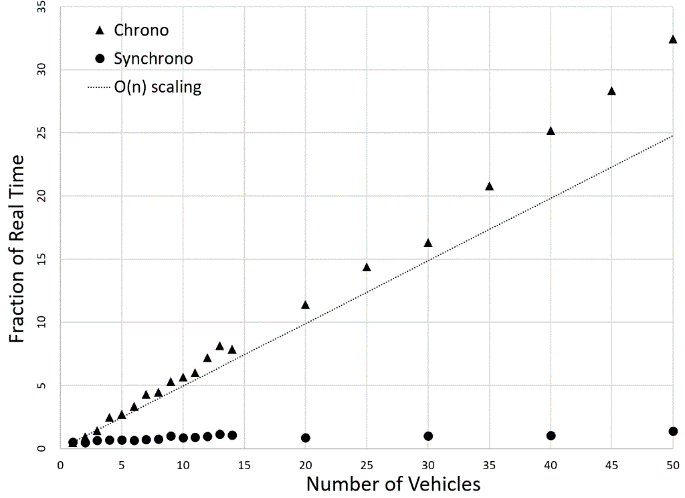
\includegraphics[width=0.8\columnwidth]{Figs/Syn-Chrono-Scaling.png}
	\caption{{\small Scaling comparison between \chrono{} and \synchrono{}. By running each simulation in parallel \synchrono{} handles scenarios with large numbers of vehicles much faster and closer to real-time than \chrono{}.}}   
	\label{fig:synchronoscalingold}
\end{figure}

\begin{figure}
	\centering
	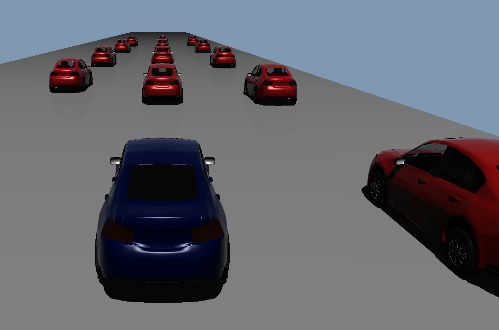
\includegraphics[width=0.8\columnwidth]{Figs/Syn-Platoon.png}
	\caption{{\small Image of a collection of agents in a shared, coherent virtual world.}}   
	\label{fig:synplatoonold}
\end{figure}

\subsection{ROS \chrono{} Control Interface}\label{s:roscontrolinterface}

To allow for the seamless testing of control algorithms that are intended to be easily transferred to real vehicles or robots, the toolset provides a \ros{} control interface that is exposed in \synchrono{}. Using \tcp{}, messages from \synchrono{} (i.e. sensor data packets), are sent into a \ros{} node on the same system running the vehicle control stack. This node also listens to the \ros{} control messages that are produced and sends them back to \synchrono{} for input to the \chrono{} agents. With this \ros{} interface, the tested control stack is independent of the \synchrono{} platform (i.e. can be run on a different operating system or architecture) and can be tested with inputs replicating those from reality, such as sensor and/or V2X communication data.

\clearpage

%% ============================================================
\section{Demonstration}\label{s:demonstration}
\todo[inline]{Asher's details on the proposed demonstration: the goal of the demonstration is to show a multi-agent simulation of vehicles driven with policies learned using RL in PyChrono. To accomplish this we will train a single agent to participate in a follow-the-leader convoy through a narrow path. It will be trained on rigid terrain until an optimal policy is found. We can then refine the policy on SCM terrain. The trained policy will be deployed for all vehicles in SynChrono. We can remove the need for sensing the SCM terrain if we using a simulated vehicle-to-vehicle message from the lead vehicle. I think it would be more interesting to include a camera as input and remove the need to know the position of the lead vehicle. Final decision on that TBD. The study will then be on how that policy is deployed in SynChrono and how it responds to perturbations in the form of ruts in the soil.}

\todo[inline]{DN - Training for convoy vehicle: sensor (GPS+Camera) fusion + rigid terrain + ghost vehicle(s). Training for lead vehicle: path (perhaps way points) + sensor fusion + obstacles}

\todo[inline]{DN: SynChrono scaling analysis on SCM with 1, 2, 4, 8, etc. vehicles; half going NS, half EW. SCM deformable terrain; deformable terrain shown in simulation and also picked up by sensor.}

%% ============================================================

\begin{figure}
    \centering
    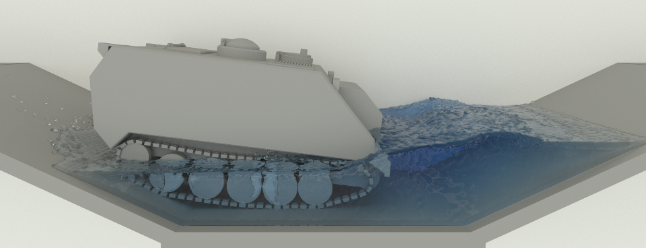
\includegraphics[width=0.8\columnwidth]{Figs/M113Fording.png}
    \caption{{\small M113 fording maneuver demonstrating \chrono{} and \chronomod{Vehicle} capabilities.}}   
    \label{fig:m113fording}
\end{figure}

\begin{figure}
    \centering
    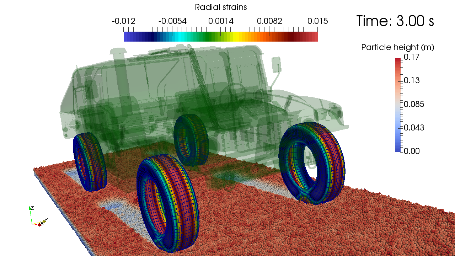
\includegraphics[width=0.8\columnwidth]{Figs/HMMWV-Granular.png}
    \caption{{\small HMMWV with flexible tires navigating granular terrain demonstrating vehicle dynamics, flexible body dynamics, and parallel computing support in \chrono{}.}}   
    \label{fig:hmmwvgranular}
\end{figure}

\begin{figure}
    \centering
    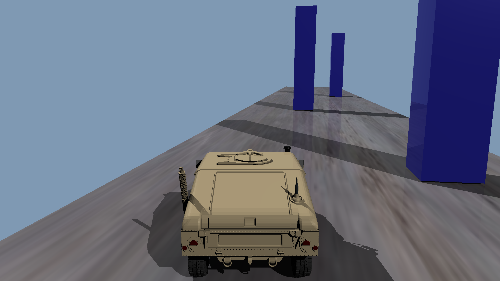
\includegraphics[width=0.8\columnwidth]{Figs/GymChrono-Pilars.png}
    \caption{{\small \gymchrono{}-enabled learning with simulated sensor data provided by \chronomod{Sensor} gradually allows the vehicle to understand how to avoid random obstacles placed in its path}}   
    \label{fig:gymchronopillars}
\end{figure}


This contribution outlines the current state of a BSD3 open-source simulation toolset whose goal is to assist practitioners in endowing autonomous agents with artificial intelligence; i.e., producing control strategies that enable heterogeneous teams of robots and wheeled/tracked vehicles to operate in off-road conditions in a coordinated fashion towards accomplishing a shared task. The toolset draws on: \chrono{} , which provides multi-physics support for agent modeling; \chronomod{Sensor}, which produces synthetic data for simulating sensing; \pychrono{} and \gymchrono{}, which provide support for machine learning; \synchrono{}, a software component for software/hardware/human in the loop studies that include multiple agents; and the \ros{}-\chrono{} Control Interface, which allows the toolset to converse with the software libraries/utilities provided by \ros{} . The reinforcement learning (RL) support provided through \gymchrono{} is demonstrated in conjunction with an RL experiment in which a HMMWV-type vehicle learns how to avoid road obstacles while moving in a convoy.


\section*{Acknowledgments}
This work was supported by a U.S. Army TARDEC project. \chrono{} development was supported in part by U.S. Army TARDEC Rapid Innovation Fund grant No. W911NF-13-R-0011, Topic No. 6a, ``Maneuverability Prediction''. 







%% *******************************************************************
%% Examples for including single- and double-column figures and tables
%% *******************************************************************

%\begin{figure}
%	\centering
%	\includegraphics[width=0.8\columnwidth]{Figs/hmmwv_1.png}
%	\caption{{\small A figure spanning a single column. The caption should wrap nicely here.}}   
%	\label{fig:one}
%\end{figure}

%\begin{figure*}
%	\centering
%	\includegraphics[width=0.75\textwidth]{Figs/hmmwv_1.png}
%	\caption{{\small A figure spanning the entire paper width}}    
%	\label{fig:two}
%\end{figure*}

% \begin{table}
% \begin{center}
% 	\begin{tabular}{||c |c | c||} 
% 		\hline
% 		Test  & Terrain  & Controller Vehicle \\
% 		Number &  Type & Model\\ [0.5ex] 	
% 		\hline\hline
% 		1 & Rigid & 2-DOF \\ 
% 		\hline
% 		2 & Rigid & 14-DOF \\
% 		\hline
% 		3 & Granular & 2-DOF \\
% 		\hline
% 		4 & Granular & 14-DOF \\
% 		\hline
% 	\end{tabular}
% \end{center}
% \caption{A table spanning a single column. The caption should wrap nicely here.}
% \label{t:one}
% \end{table}

% \begin{table*}
% 		\centering
% \begin{tabular}{ ||p{6cm}|p{1.8cm}|p{1.8cm}|p{1.8cm}|p{1.8cm}||  }
% 		\hline
% 		Test Number & 1 & 2 & 3 & 4\\
% 		\hline
% 		Controller Model & 2-DOF & 14-DOF & 2-DOF & 14-DOF\\
% 		\hline
% 		Terrain & Rigid & Rigid & Granular & Granular\\
% 		\hline
% 		Time to Target (s)  & 26.67 & 26.15 & 28.32 & 28.03\\ 
% 		\hline
% 		Minimum Obstacle Distance (m) & 0.897 & 5.462 & 3.491 & 4.721\\
% 		\hline
% 		Controller Effort & 0.0340 & 0.0340 & 0.0340 & 0.0306\\
% 		\hline
% 		Max. Lateral Acceleration (m/s$^{2}$)& 2.78 & 1.57 & 2.47 & 2.33 \\
% 		\hline
% 		Avg. Lateral Acceleration (m/s$^{2}$) &0.54 & 0.51 & 0.55 & 0.46\\
% 		\hline
% \end{tabular}
% \caption{A table spanning both columns.}
% \label{t:two}
% \end{table*}
